\documentclass[10pt,a4paper]{article}
\usepackage[utf8]{inputenc}
\usepackage{amsmath}
\usepackage{amsfonts}
\usepackage{amssymb}
\usepackage{tikz}
\usepackage{graphicx}
\author{James Lee}
\title{8th Assignment of Computational Physics}
\begin{document}
	\maketitle
	\begin{abstract}
		In this report I present to you the numerical solution to Problem 3.7.
	\end{abstract}
	\section{Introduction}
	This program aims to compute the motion of linear forced pendulum with friction using Euler-Cromer method.\\
	Oscillational motion plays a crucial role in physics, for many motions can be investigated as oscillational models. Furthermore, the solution to oscilltional motion is well known to physicists for several decades.\\
	The object we encounter here is a forced pendulum with friction. Its motion is governed by the following 2nd-order ODE:
	\begin{equation}
	\frac{d^{2}\theta}{dt^2}=-\frac{g}{l}\theta-q\frac{d\theta}{dt}+F_{D}\sin{(\Omega_Dt)}
	\end{equation}
	It is elementary for us to give the steady state solution to this ODE:
	\begin{equation}
	\theta(t)=\theta_0\sin{(\Omega_Dt+\phi)}
	\end{equation}
	where:
	\begin{equation}
	\theta_0=\frac{F_D}{\sqrt{(\Omega^2-\Omega_D^2)^2+(q\Omega_D)^2}}
	\end{equation}
	This expression indicate the existence of \emph{resonance}.\\
	It is not difficult to see that when$\Omega=\Omega_D$, the amplititude of steady state is particularly large:
	\begin{equation}
	\theta_{0\text{max}}=\frac{F_D}{q\Omega_D}
	\end{equation}
	In the following sections, I will solve the ODE in numerical approach. Furthermore, I will verify the existence of resonance.
    \section{Main Content}
    \subsection{Euler-Cromer Method}
    I will use Euler-Cromer method to solve this set of ODE.\\
    The Euler-Cromer method is a modified version of Euler method. The basic algorithms can be written as following:
    \begin{align}
    x_{n+1} &= x_n + f(t_n, v_n) \, \Delta t\\
    v_{n+1} &= v_n + g(t_n, x_{n+1}) \, \Delta t
    \end{align}
    It is easy to write a program invoking Euler-Cromer method that is similar to the previous Euler method programs.\\
    In order to give a numerical solution, one should fix the parameters numerically at first:
    \begin{align}
    \Omega_D&=2.0\\
    F&=0.2\\
    q&=1.0\\
    g&=9.8\\
    l&=1.0
    \end{align}
    the initial conditions:
    \begin{align}
    \theta|_{t=0}&=0.2\\
    \omega|_{t=0}&=-0.1
    \end{align}     
    The numerical solution to this case will be plotted in figure.1.
    \begin{figure}[htbp]
    	\centering
    	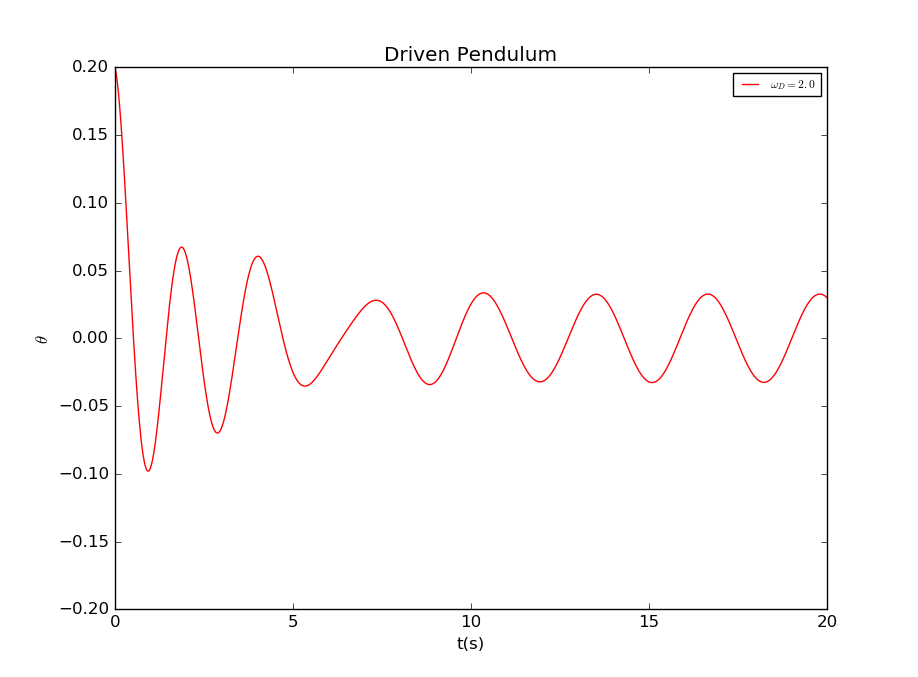
\includegraphics[width=5in]{pendulum_1.png}
    	\caption{Numerical Solutions}
    \end{figure}
    As we can see in the numerical plot figure, the forced pendulum tends to follow the motion of the external force, even with friction presents. The steady state of this pendulum is very much alike simple harmonic motion which agrees with our analytical results.\\
   \subsection{Resonance}
   Now we wish to investigate resonance behaviors.\\
   According to the previously fixed parameters, the resonance angular frequency should be:
   \begin{equation}
   \Omega_{res}=\sqrt{g/l}=3.13
   \end{equation}
   Now we set $\Omega_D=3.13$, let us have look at the numerical results:
   \begin{figure}[htbp]
   	\centering
   	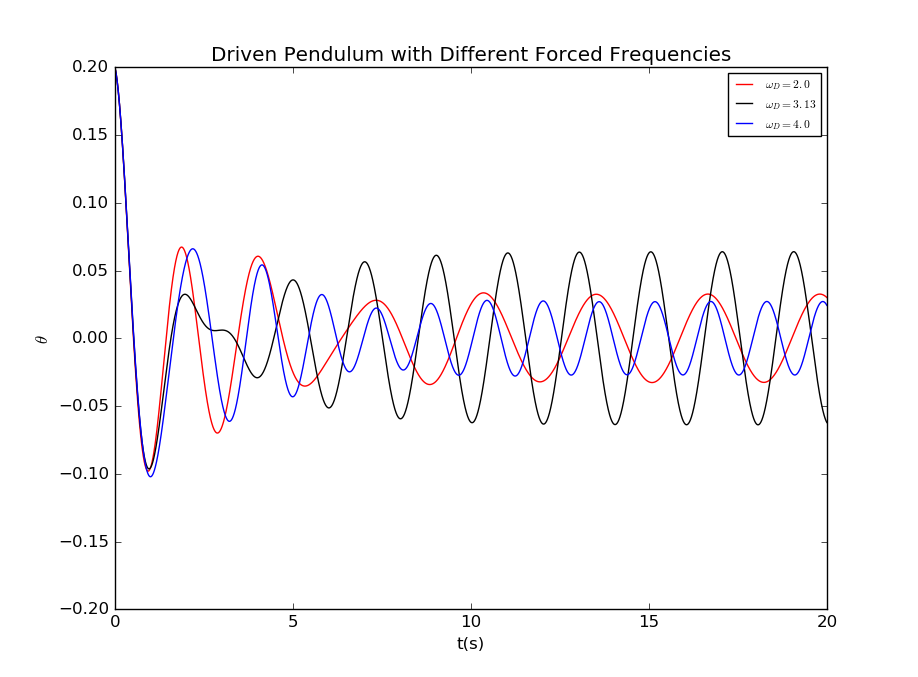
\includegraphics[width=5in]{pendulum_2.png}
   	\caption{Numerical Solutions with different $\Omega_D$}
   \end{figure}
   we can clearly see from the figure that the amplititude corresponding to resonant frequency is much larger than the other two. This figure qualitatively verify our analytical prediction of resonance.\\
   Now we want to go further to verify resonance quantitatively. In order to do that, we can set $\Omega_D$ fixed, and watch amplitude $\theta_0$ vary with the other parameter, then compare it to the theoretical curve.
    \begin{figure}[htbp]
    	\centering
    	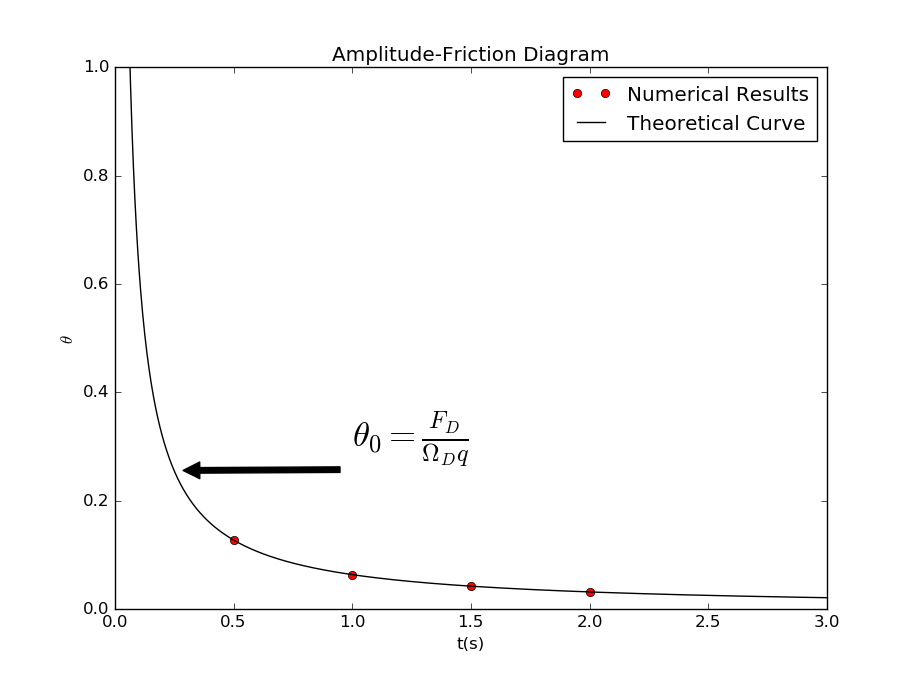
\includegraphics[width=5in]{pendulum_3.png}
    	\caption{Verification\label{Figure_3}}
    \end{figure}
     The verification to this case will be plotted in figure \ref{Figure_3}.
    As we can see in this figure, all the numerical results lie on the theoretical curve. This feature quantitatively verifies our prediction of \emph{resonance}.
    
    \section*{Acknowledgement}
    When tackling this assignment, I benefitted a lot from the valuable discussions with Liu Xingchen. I would like to thank him for pointing out several syntax errors I made, also, for his willingness to discuss with me.
    
    \begin{thebibliography}{99}
    	\bibitem{}Hunter J, the Matplotlib Documentation, 2016
    	\bibitem{}Giordano N.J, Nakanishi H, Computational Physics, Pearson Education, 2007
    \end{thebibliography} 
\end{document}